\section{Implementation of \TwoLevelIndex{}}
\label{implementation}

In this section, we show the structure we used for the \twolevelindex{} to combine the \inducedgraph{} and the \treeindex{} (Section~\ref{structure}).

\subsection{\TwoLevelIndex Structure}
\label{structure}

\begin{figure}[ht]
    \centering
    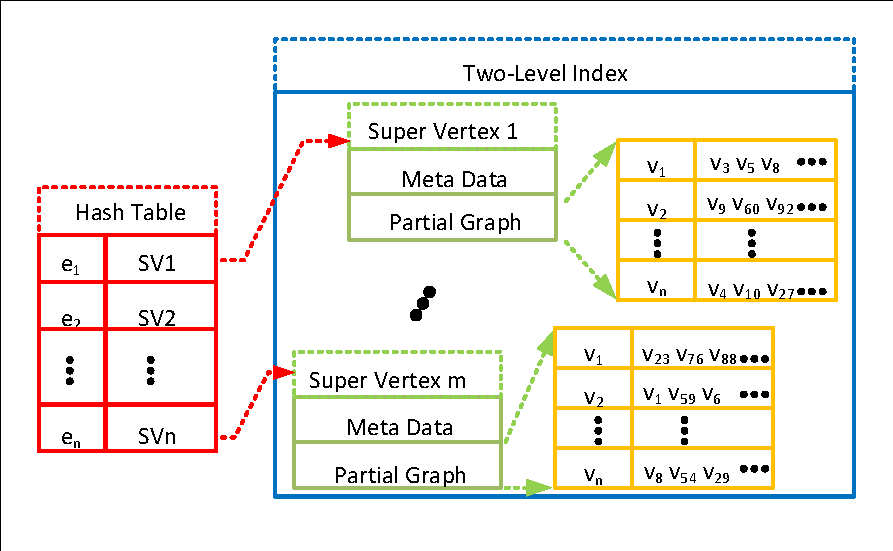
\includegraphics[width=0.8\linewidth, trim={0.1cm 0.1cm, 0.1cm, 0.1cm}, clip]{./figures/structure.pdf}
    \caption{Overall structure of the \twolevelindex{}.}
    \label{fig:structure}
\end{figure}

We combine the \inducedgraph{} and the \treeindex{} to form the \twolevelindex{} and arrange it in a structure that can provide information at different granularity. \autoref{fig:structure} shows an overview of the index structure. On the top level, we use an array to store the \treeindex{}. Each entry represents a single super vertex. Super edges are expressed by parent and children pointers. Within each entry, it also stores meta-data of the corresponding k-truss community, \eg the trussness, the community size, etc, for fast information retrieval. This meta-data can be gathered as a byproduct of index construction process. Finally, each entry contains a pointer of the data structure that stores part of the bottom level index. 

The bottom level index, which is the \inducedgraph{}, is stored as several separated adjacent lists. Each adjacent list contains edges of a single k-truss community that does not belong to any of its children k-truss communities. These adjacent lists can be easily generated as byproducts when constructing \treeindex{} using Algorithm \ref{alg:\treeindex{}_construction}.%\autoref{alg:\treeindex{}_construction}. 
%Note that a vertex or edge in the \inducedgraph{} may belong to multiple k-truss communities. In these k-truss communities, k-truss communities with higher trussness is subgraphs of k-truss communities with lower trussness. To avoid redundancy, we only store the vertex and edge in the adjacent list of the k-truss community with the highest trussness. 

Finally, we have a hash table that maps each edge in the original graph to an entry in the top level of the \twolevelindex{}. One can also follow the similar fashion used in \cite{akbas2017truss}, which maps each vertex in the original graph to multiple entries in the top level index so that the original graph is not required during query time.
